\newpage
\section{INTRODUCTION}

\thispagestyle{main}
\subsection{Introduction to the Research}
\subsubsection{Subsection}
This is the introduction to my topic. In Figure \ref{Leg} is an example of including an eps figure using the epstopdf package.

%%%%%%%%%%%%%%%%%
%  EPS Figure
%%%%%%%%%%%%%%%%%

\begin{figure}[htb]
\centering
      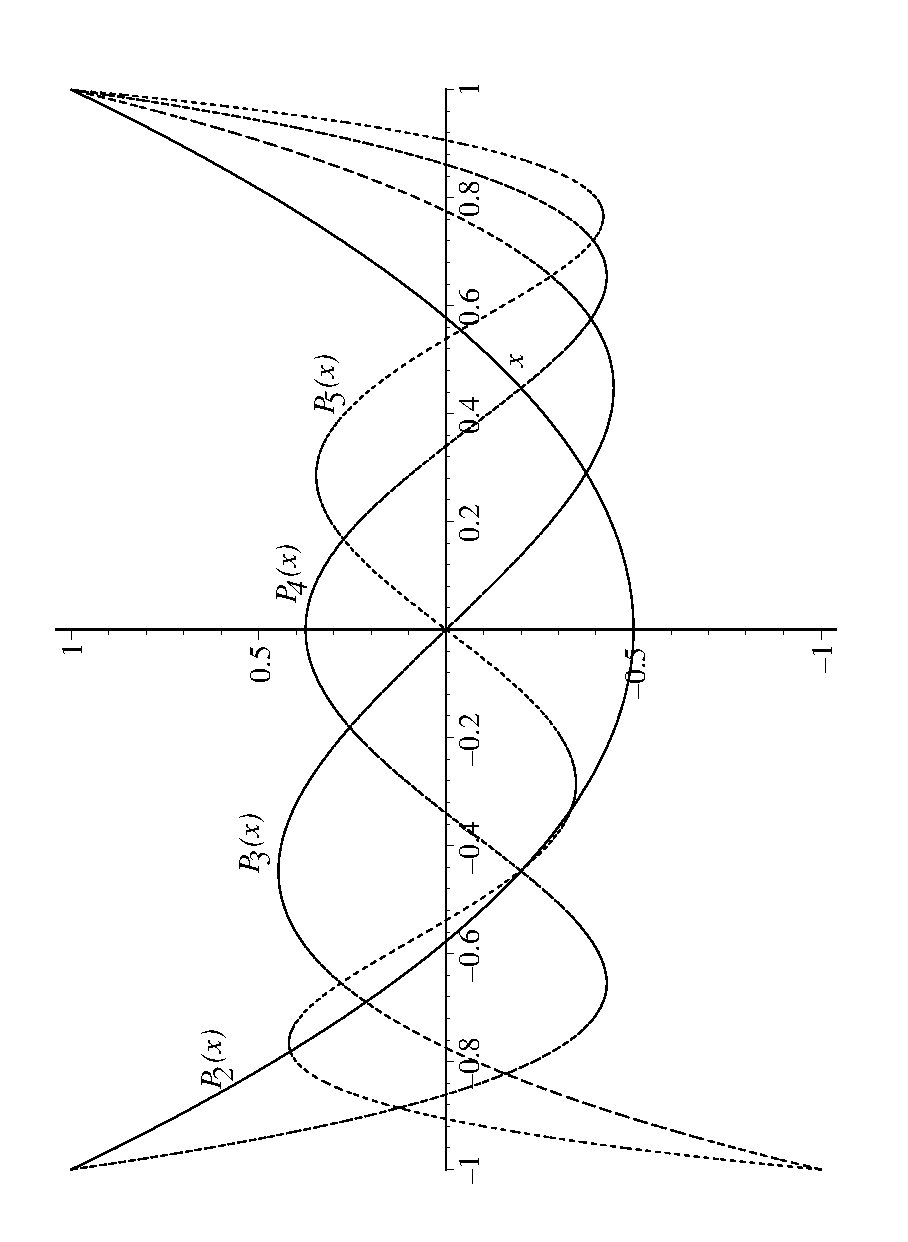
\includegraphics[width=3in,angle=-90]{images/legendre}
      \caption{Plot of Legendre polynomials. Need a longer caption to test the list of figures page. No let's see what happens.}
      \label{Leg}
\end{figure}

\lipsum[3-4]               % generates dummy text

%%%%%%%%%%%%%%%%%
%  JPG Figure
%%%%%%%%%%%%%%%%%

In Figure \ref{Fig1} we plot a jpg image.

\begin{figure}[htb]
\centering
      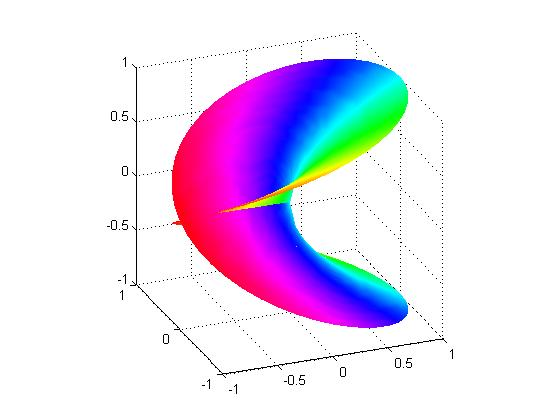
\includegraphics[width=3in]{images/RiemannSurf.jpg}
      \caption{Plot of a jpg image.}
      \label{Fig1}
\end{figure}


For definitions, theorems, and examples, you have environments which set up the proper styles. Here are examples:

\begin{definition} A {\bf foobar} is a nonsensical term.
\end{definition}

\begin{theorem} If $A=B$ and $B=C,$ then $A=C.$
\end{theorem}
\begin{proof}
This is obvious.
\end{proof}

\begin{example} Example of an example.

This is an example. 
\end{example}